 \documentclass[conference]{IEEEtran}
\IEEEoverridecommandlockouts
%\usepackage{hyphenat}
\usepackage[ruled,vlined]{algorithm2e}
\usepackage{amsmath}
\usepackage{xspace}
\usepackage[binary-units=true]{siunitx}
\usepackage{ulem}
%\usepackage{censor}
\usepackage[table]{xcolor}
\usepackage{graphicx}
\usepackage{hyperref}
\usepackage{tabularx}

\usepackage{subcaption}
\usepackage{booktabs}
\usepackage{multirow}
\usepackage{listings}
\usepackage{dingbat}

\hypersetup{
    colorlinks=true,
    linkcolor=black,
    citecolor=blue,
    filecolor=black,
    urlcolor=blue}

\def\BibTeX{{\rm B\kern-.05em{\sc i\kern-.025em b}\kern-.08em
    T\kern-.1667em\lower.7ex\hbox{E}\kern-.125emX}}


\makeatletter
  \def\footnoterule{\kern-3\p@
  \hrule \@width 2in \kern 2.6\p@} % the \hrule is .4pt high
\makeatother


\begin{document}

\newcommand{\fslspm}{FSL-SPM\xspace}
\newcommand{\fslafni}{FSL-AFNI\xspace}
\newcommand{\afnispm}{AFNI-SPM\xspace}
\newcommand{\tristan}[1]{\color{orange}\textbf{From Tristan:} #1\color{black}\xspace}
\newcommand{\ali}[2]{\color{green}\textbf{Ali:} #1\color{black}\xspace}



\title{Comparing tool variability and numerical variability in fMRI analyses}

\author{Ali Salari$^1$, Other Authors$^1$, Tristan Glatard$^1$ \\
$^1$ Department of Computer-Science and Software Engineering, Concordia University, Montreal, Canada}

\maketitle
\begin{abstract}

Numerical and software variability broadly affect structural, diffusion, and functional MRI analyses. Numerical
variability originates in software updates or code
parallelization, whereas software variability reflects discrepancies between
models implemented in different analysis software packages. While numerical
and software variability were both shown to impact analysis outcomes, the
extent to which these sources of variability compare for a given
analysis remains understudied. This work presents a comparison of
numerical and software variability for group-level functional MRI analysis
\tristan{did we give up on individual analyses?}.
We reproduced a previous comparison between functional MRI analysis
software packages FSL, AFNI, and SPM, which we extended to measure
numerical variability through Monte-Carlo arithmetic.
We find that between-tool variability is an order of magnitude higher than numerical variability.
\tristan{summarize conclusions}

\end{abstract}

\begin{IEEEkeywords}
  Numerical Instability, Reproducibility, Monte-Carlo arithmetic, Neuroimaging
\end{IEEEkeywords}


\section{Introduction}

% Data analysis workflows in many scientific domains have become increasingly complex and flexible.
Recent studies highlighted the instability of the neuroimaging pipelines depending on the computing platform,
software package, and even tool versions. Changes in the computational
environment such as compilers, libraries, operating systems may introduce small numerical errors and create
significantly different results in unstable pipelines~\cite{Glatard2015,Gronenschild2012,salari2020spot}.
Moreover, the impact of methodological changes on fMRI analyses has been investigated extensively~\cite{bowring2019exploring,botvinik2020variability,bhagwat2021understanding,carp2012plurality}.
For instance, in related works, it has been shown that running the same fMRI experiments by different teams can substantially affect
scientific conclusions~\cite{botvinik2020variability,carp2012plurality};
replication of fMRI experiments using the three most well-known software packages can influence the final determining areas of
brain activations~\cite{bowring2019exploring}; %bowring2021isolating.
also, the choice of preprocessing pipelines on neuroimaging cortical surface analyses is compound with instabilities~\cite{bhagwat2021understanding}.
% In the presence of such instabilities, it is often hard to trust the data processing results. % validity of the computational results.

In such a heterogeneous environment, numerical instability is an essential issue for reproducibility.
Numerical instability is a characteristic of pipelines that results from the influence of the floating-point arithmetics
and iterative convergence of numerical errors~\cite{freitas2002issue}.
Stochastic arithmetic approaches such as Monte-Carlo arithmetic (MCA)~\cite{Parker1997-qq} have been used to study the impact of numerical errors
originating in floating-point computations in mathematical libraries.
In~\cite{salari2021accurate}, we quantified the numerical stability of the HCP preprocessing pipeline~\cite{glasser2013} based on the MCA method
by creating a Fuzzy environment, so that instrument mathematical functions are implemented in mathematical system libraries.
As a result of numerical perturbations, we discovered a very low numerical precision in the result images comparable to the operating system variability.
In a related study~\cite{kiar2020numerical}, the instability of results was explored by instrumenting a connectome estimation pipeline with the MCA technique.
These works demonstrate the necessity of numerical uncertainty quantification for understanding related issues that hamper the computational reproducibility of analyses.

In this work, we reproduce an fMRI analysis in~\cite{bowring2019exploring} with different neuroimaging software packages in the presence of the Fuzzy environment,
and then quantify the variability across tools and the numerical variability in results.
We call the cross-software variation and numerical variation, between tool (BT) and within tool (WT) variability, respectively.
In fact, the WT variability shows results across software packages in the Fuzzy environment.
The primary objective of this study is to answer these two questions: 1) how the fMRI analyses across tools are numerically stable?
2) how the numerical variability is in comparison with the tool variability?
This comparative study reveals the importance of numerical variability and motivates research studies to evaluate the numerical uncertainty of the pipelines.

% We start to reproduce an analysis from Bowring, this can be as a practice for reproducibility manner in the community.
% In particular, we investigate the effect of 1) between software 2) within software (numerical)
% We present a comparative assessment of group-level analysis of an fMRI pipeline.


\section{Materials and Methods}

\subsection{fMRI analysis \& Dataset}

We replicated the fMRI analysis described as study `ds000001'
in~\cite{bowring2019exploring} \tristan{check if this dataset was acquired
and analysed previously, and if so cite the original paper}, relying on the
data publicly available in OpenNeuro at
\url{https://openneuro.org/datasets/ds000001} and using the three main
software packages for fMRI data processing, namely FMRIB Software Library
(FSL)~\cite{jenkinson2012fsl}, Analysis of Functional NeuroImages
(AFNI)~\cite{cox1996afni}, and Statistical Parametric
Mapping(SPM)~\cite{penny2011statistical}. We selected this dataset because
comparable analysis pipelines implemented in FSL, AFNI and SPM 
were already published and extensively described in~\cite{bowring2019exploring}.
Furthermore, the work in~\cite{bowring2019exploring} already evaluated the effect of tool variability for
this dataset, which we intended to complement with the present quantification of numerical variability.

In the selected study, 16 healthy adult subjects participated in the
balloon analog risk task \tristan{cite the task specifically} to measure
risk-taking behavior over three scanning sessions \tristan{cite the
original study (not Alex')}. We reused the preprocessing, first-level, and
second-level analyses implemented by~\cite{bowring2019exploring} consistently across all three software packages using 
widely accepted analytical steps. Table~\ref{table:pipeline-steps} summarizes the analytical steps in each pipeline.
More details are available in~\cite{bowring2019exploring,schonberg2012decreasing} \tristan{cite only one ref, the one that gives the right details}.


%%%%%%%%%% Summary of statstics %%%%%%%%
\setlength{\tabcolsep}{4pt}
\begin{table}[h]
    \centering
    \begin{tabular}{|c|l|c|c|c|}
        \hline
%        \multirow{2}{*}{} & \multicolumn{1}{c}{Thresholded}& & \multicolumn{1}{c}{Unthresholded}& \\
        \multicolumn{2}{|c|}{} & FSL & AFNI & SPM \\
        \hline
        {Preprocessing} & {Motion Correction}                          & \checkmark    & \checkmark     & \checkmark  \\
        {} & {Segmentation}                               &    &      & \checkmark  \\
        {} & {Brain Extraction (Anatomical)}              & \checkmark     & \checkmark    & \checkmark  \\
        {} & {Brain Extraction (Functional)}              &   & \checkmark     &  \\
        {} & {Intra-subject Coregistration}               & \checkmark    & \checkmark     & \checkmark \\
        {} & {Inter-subject Registration}                 & \checkmark    & \checkmark     & \checkmark \\
        {} & {Analysis Voxel Size}                        & \checkmark    & \checkmark     & \checkmark \\
        {} & {Smoothing}                                  & \checkmark    & \checkmark     & \checkmark  \\
        \hline
        {First-level} & {Model Specification}                          & \checkmark    & \checkmark     & \checkmark  \\
        {} & {Inclusion of 6 Motion Parameters}                               & \checkmark   &  \checkmark    & \checkmark  \\
        {} & {Model Estimation}                           & &     & \checkmark  \\
        {} & {Contrasts}                                   &  \checkmark & \checkmark     & \checkmark \\
        \hline
        {Second-level} & {Model Specification}                          & \checkmark    & \checkmark     & \checkmark  \\
        {} & {Model Estimation}                           &      &    & \checkmark  \\
        {} & {Contrasts}                                   &   & \checkmark     & \checkmark  \\
        {} & {Second-level Inference}                               &  \checkmark  &    \checkmark  & \checkmark  \\
        \hline

      \end{tabular}
    \caption{Software processing steps (adapted from~\cite{bowring2019exploring}).}
    \label{table:pipeline-steps}
\end{table}

\subsection{Fuzzy libmath environment}

To introduce controlled amounts of numerical error in the analyses, we used the Fuzzy Libmath (FL) library~\cite{salari2021accurate}, an MCA-instrumented 
version of the GNU mathematical library (libmath).
Using FL, we can simulate numerical variability at the level of machine error \tristan{you really shouldn't put so much emphasis on machine error so early in the description. First, explain how FL works, then, say that you used it to simulate machine error but not only.}, the floating-point rounding error
caused by floating-point representation limits defined by the hardware \tristan{this is a quite bad definition of machine error}.

FL works based on the MCA, a floating-point arithmetic that simulates roundoff and catastrophic cancellation errors
by introducing a controlled amount of noise in the floating-point operations 
through the following perturbation model~\cite{Parker1997-qq}:

\begin{equation} \label{eq:mca_inexact}
  inexact(x) = x + 2^{e_x-t}\xi
\end{equation}

where $e_x$ is the exponent in the floating-point representation of $x$,
$t$ is the virtual precision, the number of bits in mantissa that will not be perturbed,
and $\xi$ is a random uniform variable of $(-\frac{1}{2}, \frac{1}{2})$.
The MCA perturbations are automated using Verificarlo tool~\cite{denis2015verificarlo} at compilation time.

The instrumented functions are loaded in the pipeline using LD\_PRELOAD, a Linux environment variable
to force load a shared library into an executable. This allows functions defined in FL to transparently
overload the original ones without the need to modify or recompile the analysis pipeline.

FL only introduces perturbations in the output values of mathematical
functions but not in their implementation. This is done by wrapping the original functions 
and applying function \texttt{inexact} to their returned values.
Listing~\ref{algo:wrapper} shows an example of this wrapping for the log function in both single and double precisions.
In this script, the original functions are called by \texttt{dlsym},
a function that returns the memory address of a symbol, in our case \texttt{RTLD\_NEXT}, the address of the next occurrence of the function.
These wrappers are compiled with Verificarlo for each function. The MCA
instrumentation is activated by adding a floating-point zero to the output
of the original function so that this summation is instrumented.


% \lstdefinestyle{customc}{
%   belowcaptionskip=1\baselineskip,
%   breaklines=true,
%   frame=L,
%   xleftmargin=\parindent,
%   language=C,
%   showstringspaces=false,
%   basicstyle=\footnotesize\ttfamily,
%   keywordstyle=\bfseries\color{green!40!black},
%   commentstyle=\itshape\color{purple!40!black},
%   identifierstyle=\color{blue},
%   stringstyle=\color{orange},
% }

\lstdefinestyle{customasm}{
  belowcaptionskip=1\baselineskip,
  frame=L,
  xleftmargin=\parindent,
  language=[x86masm]Assembler,
  basicstyle=\footnotesize\ttfamily,
  commentstyle=\itshape\color{purple!40!black},
}
\lstinputlisting[caption=Sample wrapper script, label=algo:wrapper, style=customasm]{wrapper.c}
%\lstinputlisting[caption=Scheduler, style=customc]{../wrapper2.c}

FL allows measuring the effect of numerical variability by running a program multiple times, 
resulting in multiple independent realizations of the same analysis. Each of these samples 
are equally plausible estimates of the true numerical result. 

FL enables us to assess the software packages that are dynamically linked to the mathematical library.
So, it is important to trace the tool dependencies of the pipelines to understand the different libraries
involved during the pipeline executions \tristan{this is not methods. Here you should report how you validated the instrumentation 
of each pipeline: (1) dependency analysis, (2) runtime checks, etc}.
\subsection{Data processing}

To measure between-tool (BT) variability, we executed the pipelines described in~\cite{bowring2019exploring}
with FSL version 5.0.10, AFNI version 18.1.09, and SPM12 version r7771
executed with GNU/Octave version 5.2. \tristan{are these versions the same as in Alex' paper?} 
FSL and AFNI scripts were executed in Python 2.7 \tristan{why?}. We also used a fixed number of 7 threads in AFNI executions,
to reproduce similar results in~\cite{bowring2019exploring} in a feasible execution time.
All the analyses were conducted on the same operating system, CentOS 7.3.
We ensured that the software versions \tristan{you mentioned versions before, the writing is a bit circular here} used in all experiments were similar to the original study,
and encapsulated them in Docker container images with available Dockerfiles at \url{https://github.com/ali4006/fuzzy-neurotools/tree/main/dockerfile}.

The same subjects and analyses were conducted in the same configurations
with the FL environment, to measure within-tool (WT) variability. We
applied instrumentations at the virtual precision t=53 bits for
double-precision floating-point values and t=24 bits for single-precision
values. Three fuzzy samples were generated for each subject and tool, to
match the number of tool samples. \tristan{mention that for FSL you also used more virtual precisions}

We evaluated WT and BT variabilities in thresholded and unthresholded group-level and subject-level t-statistics maps.
We computed voxel-wise standard deviations of T-statistic values for each pair of tools
and then compared the distribution of \tristan{there's no distribution analysis in your results} standard deviations in both conditions.
We computed the WT standard deviation as the square root of the summation of variances between samples in each tool. \tristan{write it as a formula, it's important enough and will be clearer}

Moreover, we determined region-by-region Dice coefficients for the thresholded maps for each pair of tools.
We characterized 360 regions that correspond to the cortical parcellation atlas
in Human Connectome Project Multi-Modal Parcellation version 1.0 (HCP-MMP1.0)~\cite{glasser2016multi}.
Dice values in WT are computed as the average pair-wise Dices among three Fuzzy samples for each pair of tools.
Also, we compared the correlation of Dice scores normalized by the region sizes in both conditions \tristan{move to results}.

\tristan{did you check standard error vs standard deviation?}\ali{STD shows variability of data in relation to the mean (what we are looking for here),
while SE is a type of STD (computed as $\frac{\sigma}{\sqrt{n}}$) for distribution of means (we use it when we are interested in the precision of means in different samples).}


\section{Results}
All scripts and data to create the figures presented in this section are available at \url{https://github.com/ali4006/fuzzy-neurotools} \tristan{move to lab org}.
The computations were performed on \href{https://www.computecanada.ca}{Compute Canada's} Béluga cluster
with 872 nodes, each with 2× Intel Gold 6148 Skylake @ 2.4 GHz (40 cores/node) CPU and node memory ranging from 92 to 752 GB.

We ensured a successful replication of the analyses initally presented in~\cite{bowring2019exploring}
by visually checking the overlap \tristan{what do you mean ``visually checking the overlap?'' Afair we had looked at the difference images?} of T-statistic group maps.
We could replicate the analyses across tools with an exception for AFNI that produced results with slight differences \tristan{this needs discussion on how to present it}. 
This might be caused by the compiler variations, or different hardware and their optimizations
such as out-of-order execution (dynamic scheduling) paradigm~\cite{duben2014use,demmel2013numerical}.
In this paradigm, the processors might execute instructions out of the original order they appear based on
the availability of input data and execution units to use resources efficiently. Therefore, it might
compute floating-point operations in a different order, which often leads to different results \tristan{is this a compiler optimization? If so, just mention ``compiler optimizations such as dynamic scheduling'', no need to enter into details}.

Summary statistics for the group-level unthresholded and thresholded T-statistics \tristan{harmonize capitalization in ``T-statstics / t-statistics'' (t should be lower case unless it's the first word in the sentence)} are reported in Table~\ref{table:pipeline-stats}.
% The variability between results of each pair of tools in BT and individual tools in WT was measured using the mean and standard deviation of absolute differences.
Overall, WT variability was an order of magnitude lower than BT variability for both means and standard deviations.
While the highest variability was observed in \fslafni, \fslspm was made the least variations in BT.
Results also show that AFNI was generated the most variability in WT among the three tools \tristan{this needs statistical testing}.


%%%%%%%%%% Summary of statstics %%%%%%%%
\setlength{\tabcolsep}{7pt}
\begin{table}[h]
    \centering
    \begin{tabular}{cccc|cc}
        \toprule
        \multirow{2}{*}{}& {} & \multicolumn{2}{c}{Thresholded} & \multicolumn{2}{c}{Unthresholded} \\
        \cmidrule{3-4} \cmidrule{5-6} \\
        {} & {} & Mean & Std. dev. & Mean & Std. dev. \\
        \midrule
        \rowcolor{lightgray}
        {Between Tools} & FSL vs. SPM        &  0.043       & 1.282      & 0.242     & 0.443  \\
        \rowcolor{lightgray}
        {(BT)} & FSL vs. AFNI         &  0.099       & 1.548      & 0.302     & 0.547  \\
        \rowcolor{lightgray}
        {} & AFNI vs. SPM         &  0.079       & 1.475      & 0.254     & 0.608  \\
        {Within Tool} & FSL    &  0.005       & 0.354      & 0.034     & 0.082  \\
        {(WT)}   & SPM    &  0.006       & 0.252      & 0.025     & 0.054  \\
        {}   & AFNI   &  0.017       & 0.434      & 0.041     & 0.128  \\
        \bottomrule
    \end{tabular}
    \caption{Summary of voxel-wise mean and standard deviation of absolute differences in group-level T-statistics in BT and WT. \tristan{discuss this caption}}
    \label{table:pipeline-stats}
\end{table}


% \subsection{Comparing disparity in BT and WT}
%\subsection{Spatial localization of disparity in BT and WT}
\subsection{Group-level thresholded maps}

%Fig 1
Comparisons of standard deviations between thresholded images \tristan{Table II should show summary statistics from the maps, is it the case?} in WT and BT
on MNI space are shown in Figure~\ref{fig:thresh-maps}.
While we observed substantial BT variations with the average standard deviation $\approx$ 1.5 \tristan{why approx? },
the magnitude of WT variations was much lower with the average standard deviation $\approx$ 0.5,
as was anticipated. However, numerical variability was still significant in WT results \tristan{this doesn't mean much. Also, ``significant'' means ``statistically significant''.}.
%Moreover, the numerical perturbations produces variations in similar order og magnitude in WT compared to BT variations
Moreover, the magnitude of WT variations reached the magnitued of BT variations
in some regions, shown in white in Figure~\ref{fig:thresh-maps}-\textbf{C}.

% Fig2
Figure~\ref{fig:dice-thresh} compares regional normalized Dice coefficients of
activated voxels, showing a linear correlation between BT and WT \tristan{report p-value}. 
Also, small P-values across all three pairs, including \num{1e-10} for \fslafni, \num{6e-04} for \fslspm,
and \num{2e-05} for \afnispm, confirmed this correlation of similarities \tristan{are these the p values of the regressions?}.
% The vertical line where the Dice score is zero in BT demonstrates regions in the brain with no overlaps between activated voxels in BT but WT,
% including left/right `V1\_ROI'\footnote{The primary visual cortex} in \fslafni and \fslspm,
% and left/right `TGd\_ROI'\footnote{The area TG dorsal (part of lateral temporal cortex)} in \afnispm results.


%%%%%%%%%% Var. of Thresh %%%%%%%%
\begin{figure*}[ht]
    \fbox{\begin{minipage}{\dimexpr \textwidth-2\fboxsep-2\fboxrule}
      \centering
      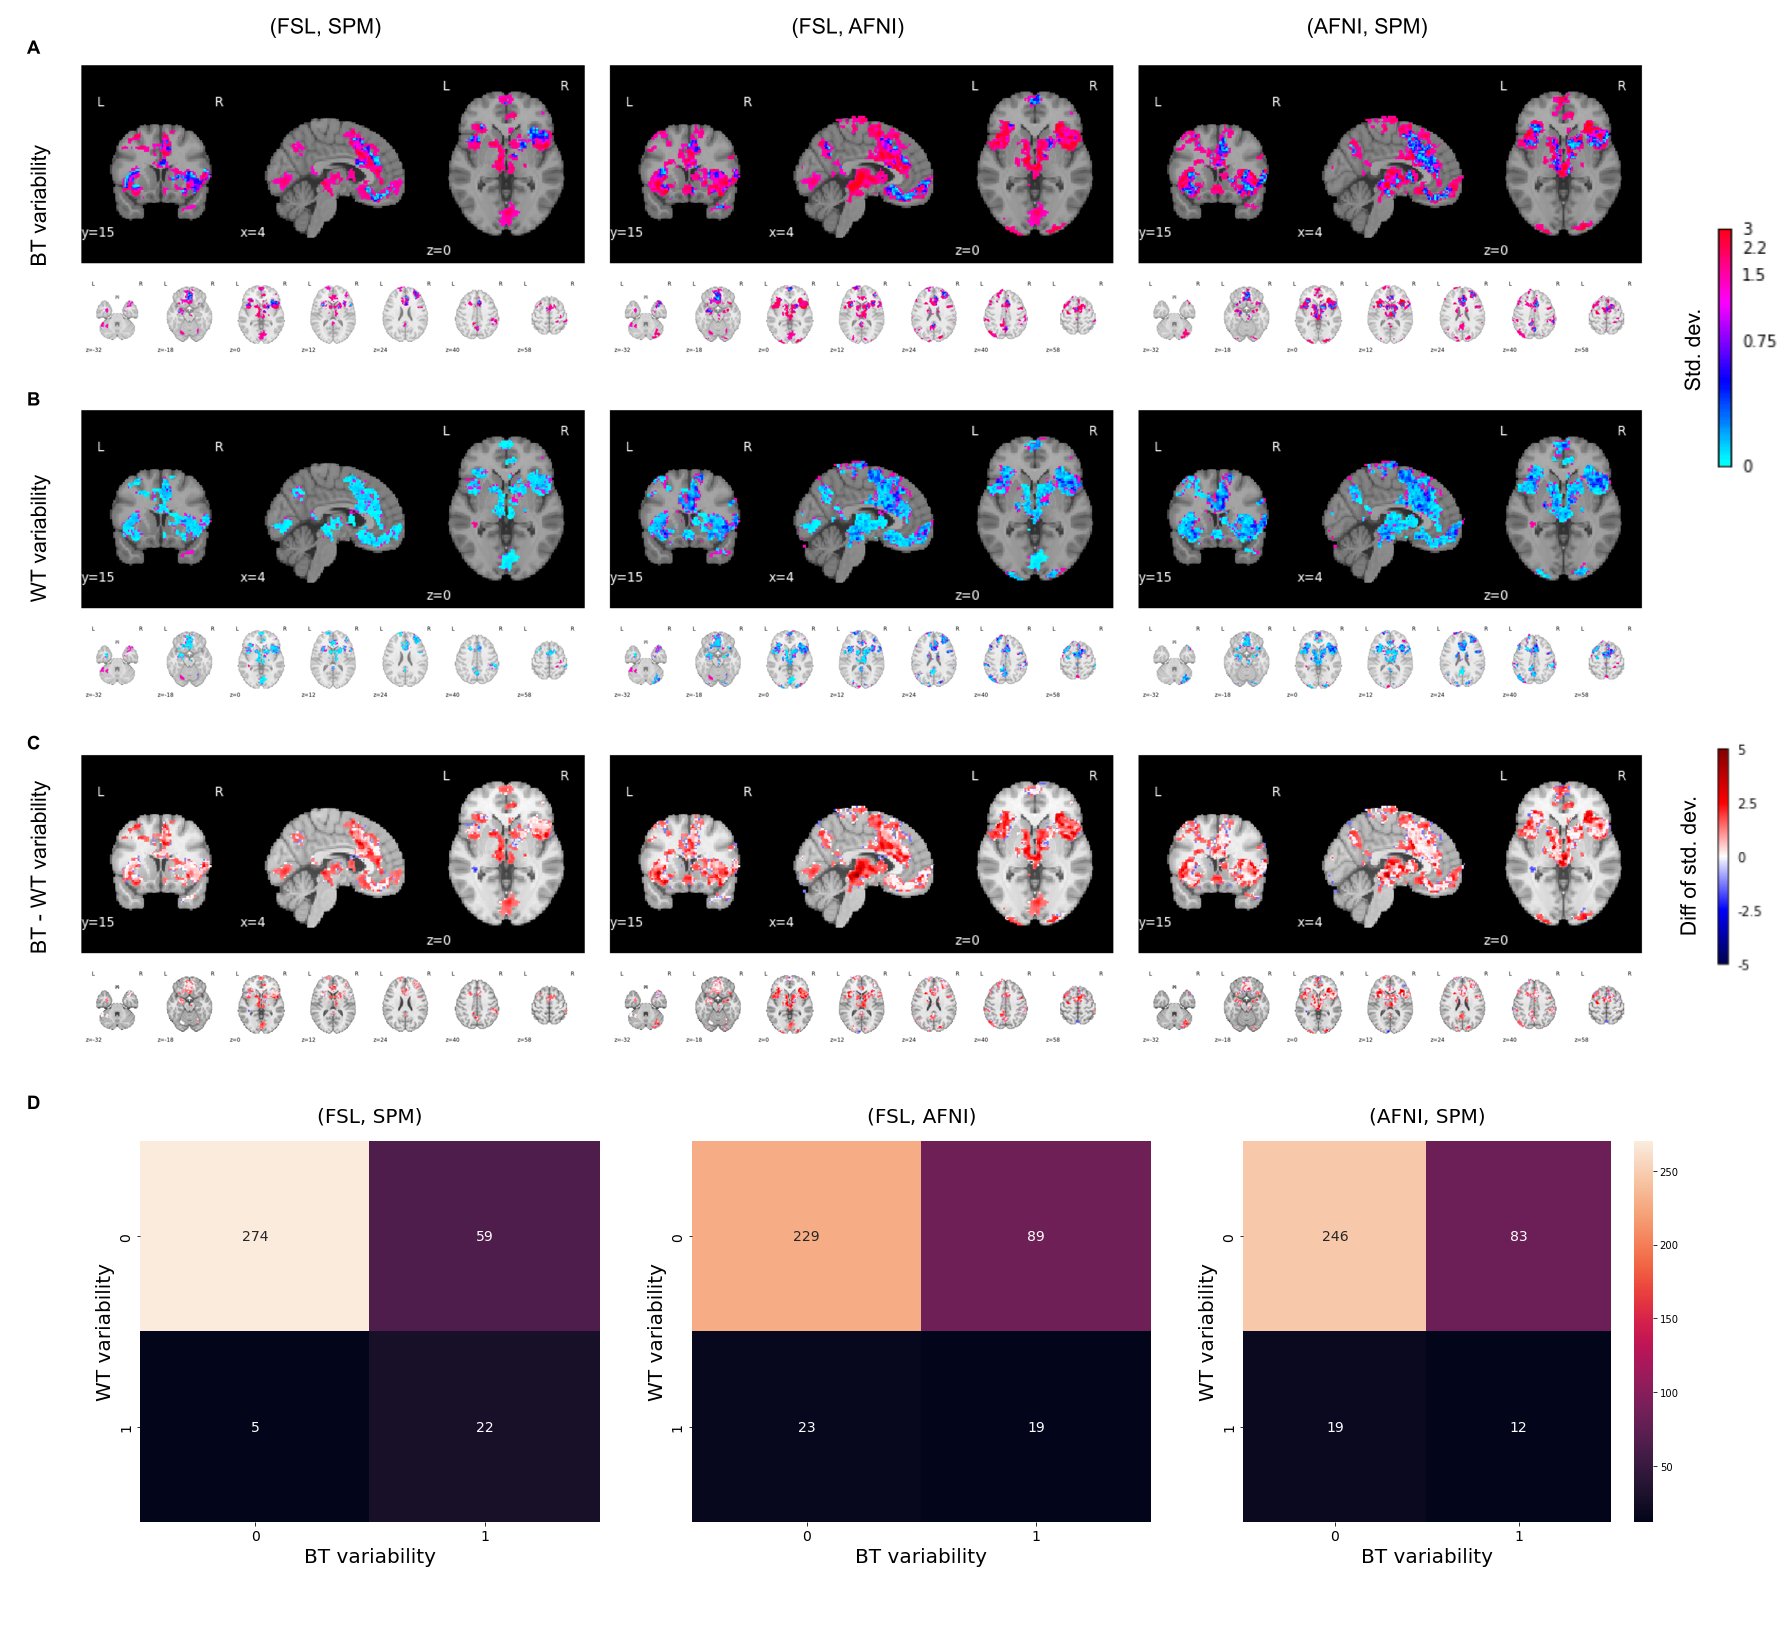
\includegraphics[width=\textwidth]{figures/std/gl-thresh.png}
      %\caption{Standard deviation of thresholded t-statistics map on template surface}
    \caption{Thresholded group t-statistics standard deviations computed between tools (\textbf{A}) and within tools (\textbf{B}), and difference between them (\textbf{C}). }
    % so that bright blue areas indicate more similar order of magnitude of variations in both conditions,
    %and vise versa for the darkder regions.}
    \label{fig:thresh-maps}
    \end{minipage}}
  \end{figure*}


  %%%%%%%%%% Dice plot of thresholded tstats%%%%%%%%
  \begin{figure}[ht]
    \fbox{\begin{minipage}{\dimexpr \columnwidth-2\fboxsep-2\fboxrule}
    \centering
    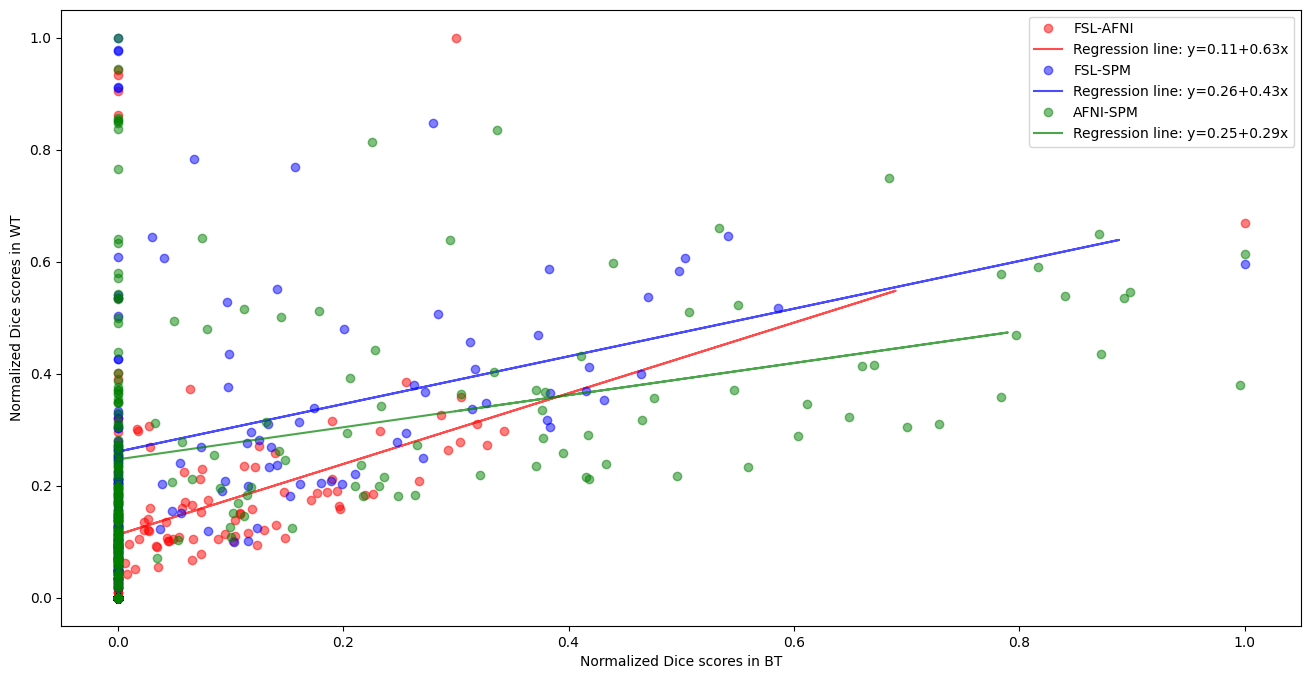
\includegraphics[width=\columnwidth]{figures/dices_corr.png}
    \caption{Normalized, regional Dice coefficients of activated voxels for
    BT and WT using the HCP-MMP1.0 parcellation of
    ~\cite{glasser2016multi}.}
    \label{fig:dice-thresh}
    \end{minipage}}
  \end{figure}



\subsection{Group-level unthresholded maps}
% \subsection{Variability of unthresholded statistical maps}

% Fig3
Similar conclusions are drawn from the unthresholded t-statistcs maps
(Figure~\ref{fig:unthresh-maps}). BT variability is an order of magnitude
higher than WT variability overall, however, BT and WT variability are
comparable in some regions. 

% shows the brain maps of standard deviations for group-level unthresholded
% T-statistics in WT and BT. Results show a different order of magnitude of
% variations in WT and BT with standard deviation of $\approx$ 0.12 and
% $\approx$ 0.5 on average, respectively. We observed regions in the brain
% where the magnitude of standard deviation was close to zero in WT, but it
% exceeded 2.0 in BT, such as some parts of the limbic and frontal lobes in
% the sagittal plane. However, the brain maps included voxels with
% approximately zero differences of standard deviations in WT and BT, which
% are uniformly distributed.

%%%%%%%%%% Var. of Unthresh %%%%%%%%
\begin{figure*}[ht]
    \fbox{\begin{minipage}{\dimexpr \textwidth-2\fboxsep-2\fboxrule}
      \centering
      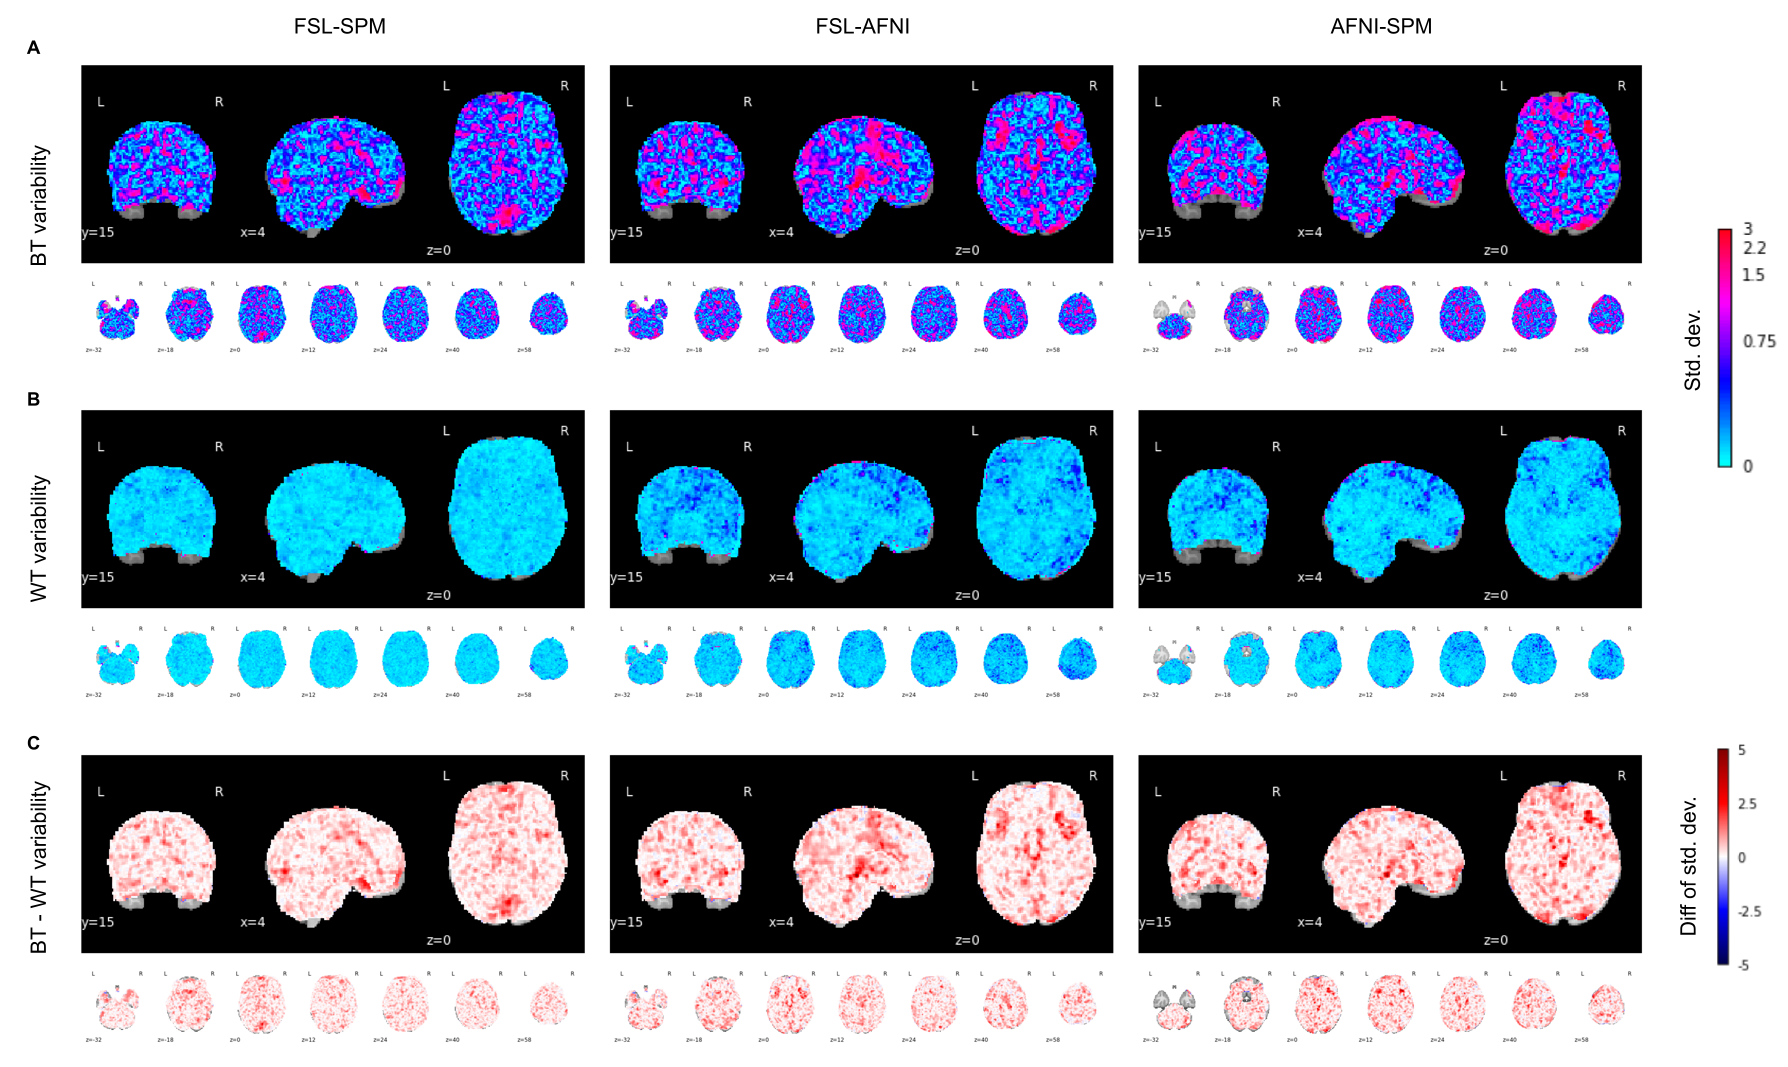
\includegraphics[width=\textwidth]{figures/std/gl-unthresh.png}
      %\caption{Standard deviation of thresholded t-statistics map on template surface}
    \caption{Unthresholded group t-statistics standard deviations computed between tools (\textbf{A}) and within tools (\textbf{B}), and difference between them (\textbf{C}).}
    \label{fig:unthresh-maps}
    \end{minipage}}
  \end{figure*}


% Fig4
\tristan{rewrite this paragraph}
The scatter plot in Figure~\ref{fig:unthresh-correlation} represents the correlation of standard deviation in WT and BT variability.
We found two major clusters, including the identity cluster that corresponds to the correlations
between BT and WT with the ratio of $0.5 < BT/WT < 2$ where the standard deviations were bigger than 0.1,
and the upper cluster that shows voxels where BT $\approx$ 0.
The percentage of voxels included in the identity cluster was \%9.9 in \fslspm, \%17.3 in \fslafni, and \%13.8 in \afnispm,
and in the upper cluster was $\approx$ \%1 for each pair of tools.
The identity area is also represented on the MNI space in the second row in Figure~\ref{fig:unthresh-correlation}.
This figure shows the spatial localization of the parts of the brain that BT variability was correlated with the numerical variability.
This refines the presented results in Figure~\ref{fig:unthresh-maps},
which indicated how the correlation is uniformly distributed across the brain.

  %%%%%%%%%% Corr. plot of tstats%%%%%%%%
  \begin{figure*}[ht]
    \fbox{\begin{minipage}{\dimexpr \textwidth-2\fboxsep-2\fboxrule}
      \begin{subfigure}[ht]{\textwidth}
        \centering
        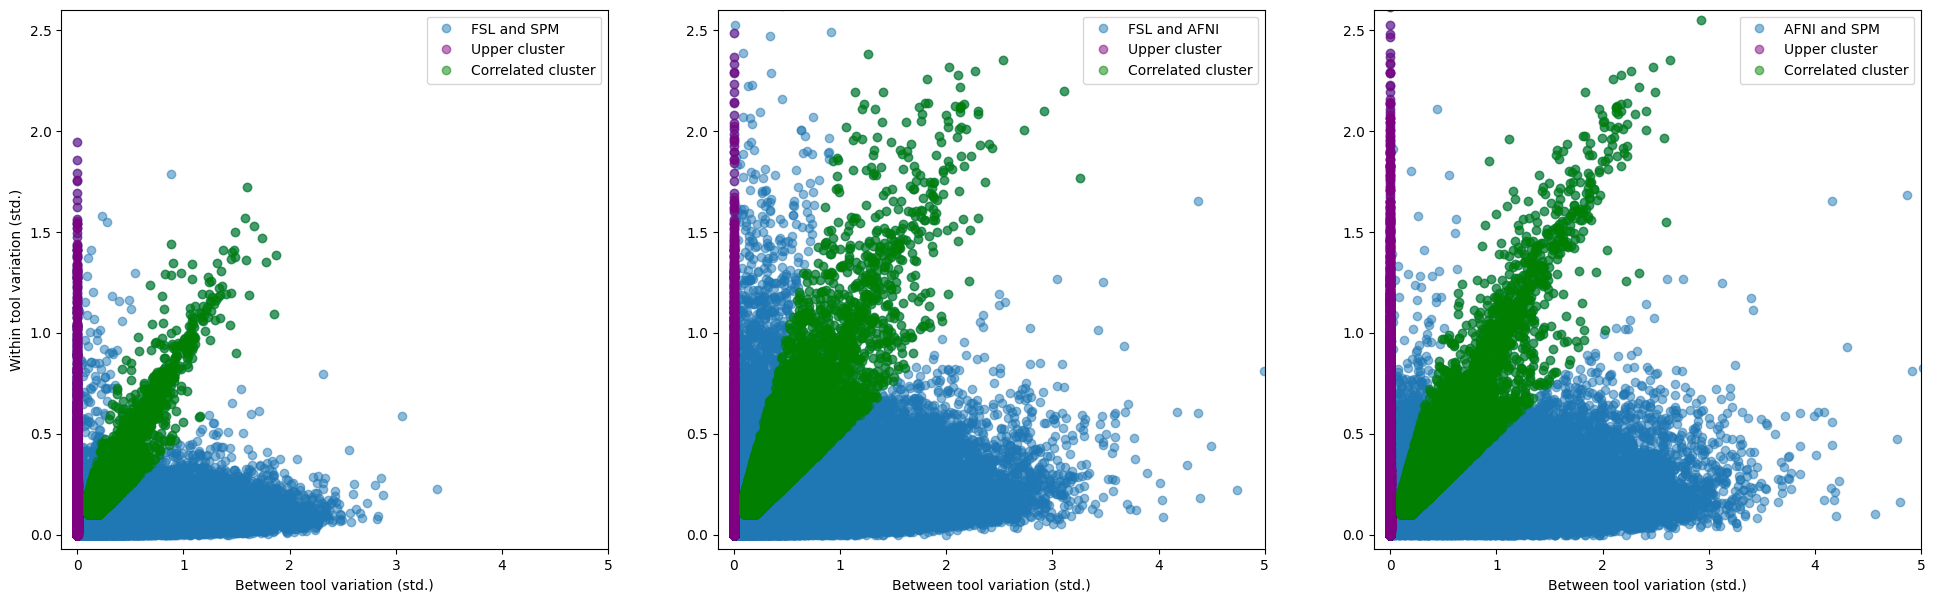
\includegraphics[width=\textwidth]{figures/std-corr-unthresh-plot.png}
        %\caption{Standard deviation of thresholded t-statistics map on template surface}
      \end{subfigure}
      \hfill
      \begin{subfigure}[ht]{\textwidth}
        \centering
        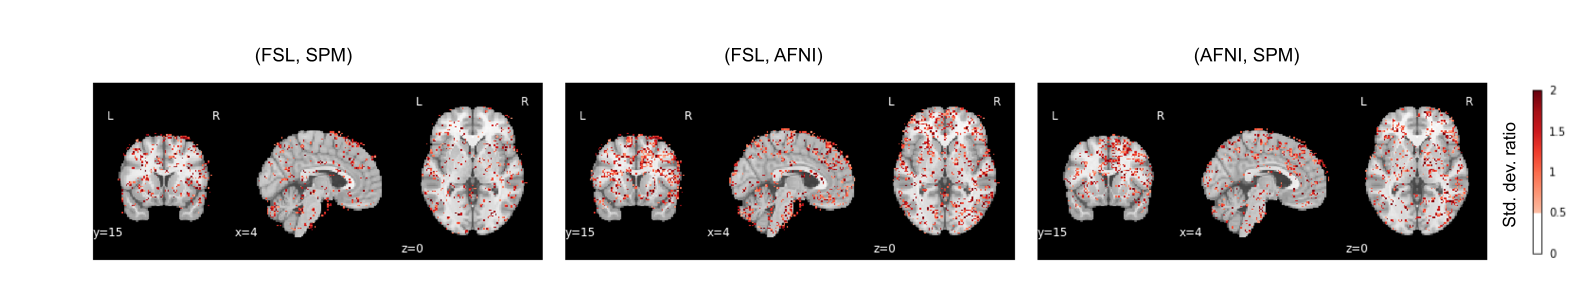
\includegraphics[width=\textwidth]{figures/std/correlated-unthresh.png}
        %\caption{Standard deviation of thresholded t-statistics map on template surface}
      \end{subfigure}
      \caption{Correlation of standard deviations in BT and WT from the unthresholded T-statistics.
      The first row plots the correlations voxel by voxel and is highlighted with different colors
      for two clusters, including the upper cluster (purple color) and the correlated cluster (green color).
      The second row maps the correlated area on the MNI space. \tristan{Fix colors and captions (to be discussed)}}
    \label{fig:unthresh-correlation}
    \end{minipage}}
  \end{figure*}


  \subsection{Subject-level unthresholded maps}

  % Table~\ref{table:firstlevel-stats} shows a summary of the statistics from the subject-level analysis results.
  % This table represents the average of the mean and standard deviation of absolute differences of unthresholded T-statistics
  % across 16 subjects for each pair of tools.
  % Results show the subjects that were produced the least and the most variability among all pairs, subjects,
  % and both BT and WT.
  % While the subject with the least variability generated results with the mean of $\approx$ 0.093 and standard deviation of $\approx$ 0.174,
  % the subject with the most variability produced results with the mean of $\approx$ 0.183 and standard deviation of $\approx$ 0.341.
  % This observation shows an order of magnitude of variability between subjects.

  Figure~\ref{fig:unthresh-maps-sbj} shows BT and WT variability of the
  unthresholded t-statistics for the subject with the highest WT
  variability among the 16 subjects. The average standard deviation for
  this subject was $\approx$ 0.152 for WT and $\approx$ 0.466 for BT
  \tristan{remove $\approx$, discuss what these numbers represent}.
  As can be seen in the Figure, WT variability approaches and even surpasses BT variability in some regions.
  

  %%%%%%%%%% Var. of Unthresh sbj05%%%%%%%%
\begin{figure*}[ht]
  \fbox{\begin{minipage}{\dimexpr \textwidth-2\fboxsep-2\fboxrule}
    \centering
    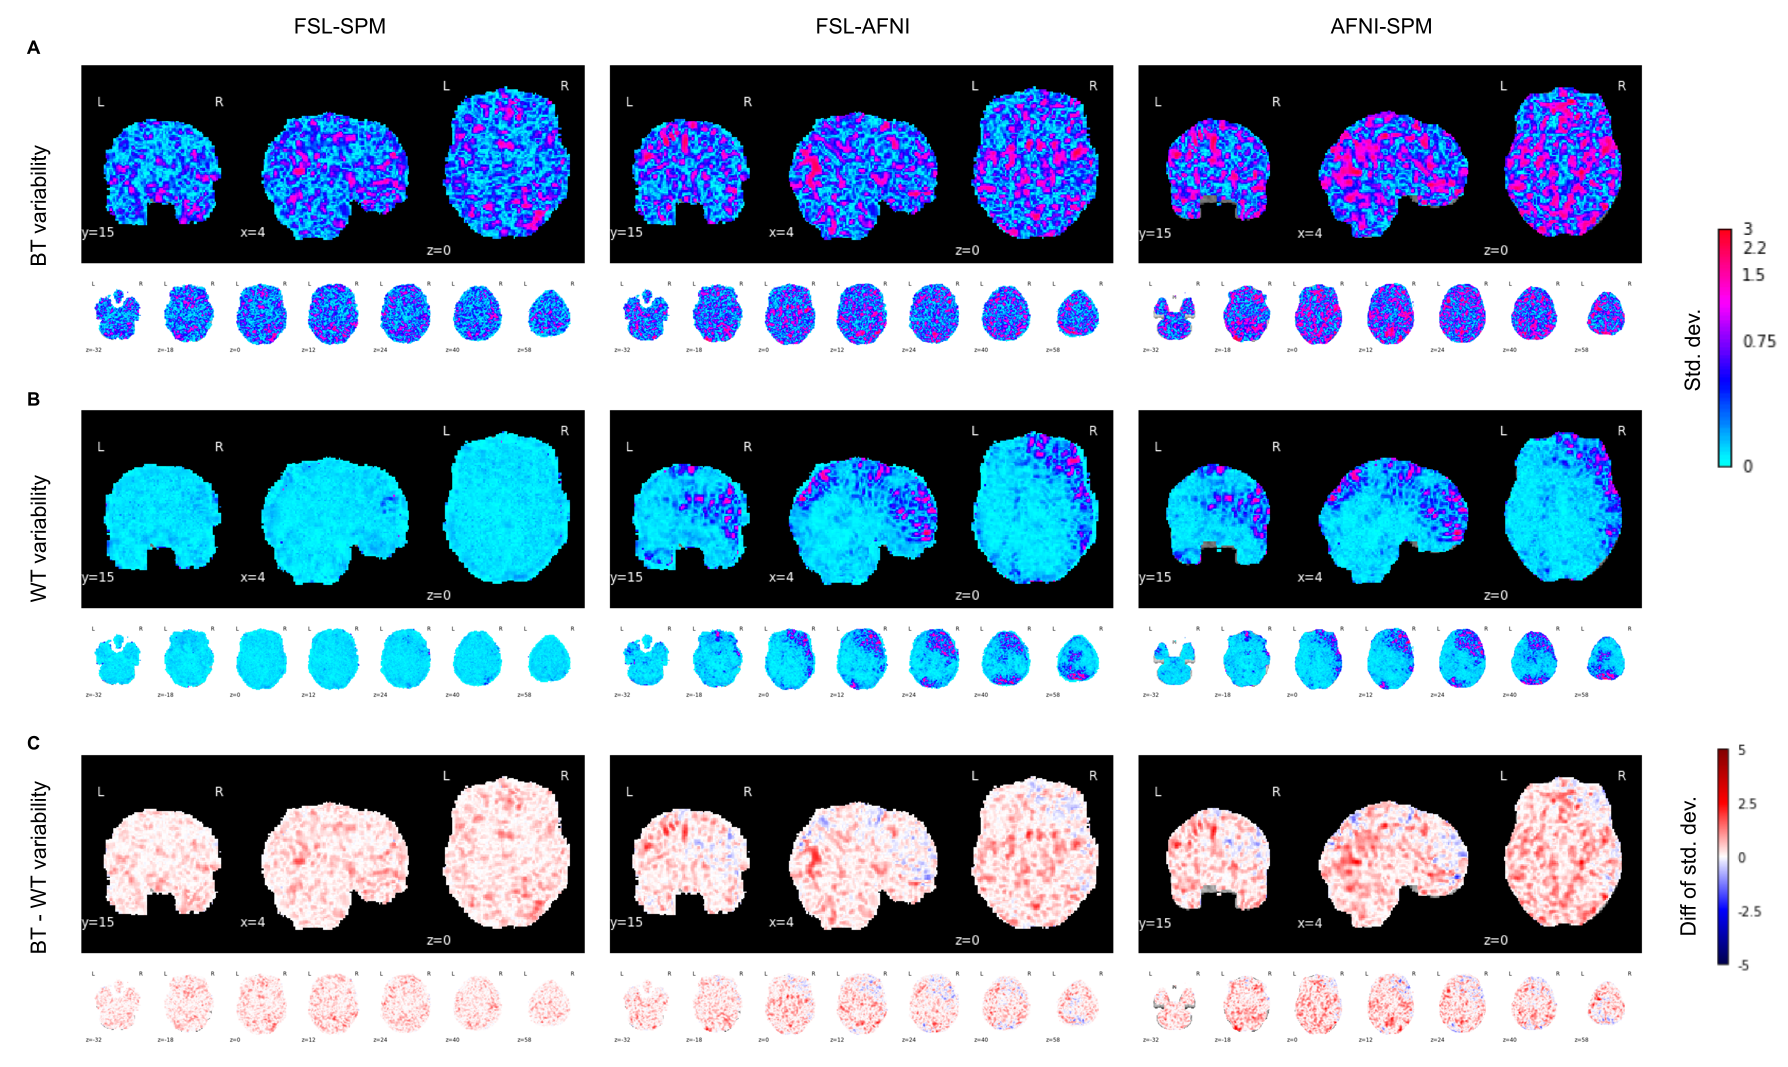
\includegraphics[width=\textwidth]{figures/std/sbj05-std.png}
    %\caption{Standard deviation of thresholded t-statistics map on template surface}
  \caption{Maps of standard deviation of unthresholded T-statistics in subject 5. The first and second rows show
  maps on BT and WT results, respectively, and the third row represents maps of their differences.}
  \label{fig:unthresh-maps-sbj}
  \end{minipage}}
\end{figure*}

\subsection{WT variability across virtual precisions}

While the previous results were obtained at the virtual precision of 53~bits for double-precision floating-point values
and 24~bits for single-precision values, we evaluated WT variability across different virtual precisions for FSL. \tristan{make sure this is described in the methods}
Figure~\ref{fig:across-precisions} represents the RMSE between standard deviations of each pair of tools in BT and FSL variations across virtual precisions in WT \tristan{clarify what is shown}.
%Consistant with the previous results, 
RMSE between WT and BT for \fslafni was the highest, and \fslspm was the lowest in all virtual precisions.
This also shows the similar plateaus were generated in all three pairs of tools.
Moreover, the analyses crashed for the precisions below t=11 bits during the FSL preprocessing steps. 
This needs further investigations to understand the exact failure reasons. 

\tristan{make a full figure, similar to Fig 1, 3, and 5. }We determined the virtual precision of t=27 bits as the precision that minimized the RMSE between standard deviations in BT on average and WT.
This is the precision that numerical perturbations in FSL more closely simulated BT variability.
Figure~\ref{fig:gnp-mni} shows the brain maps of numerical variability obtained from the analysis with FSL at t=27 bits.
This represents regions with significant variability in the frontal, parietal, and limbic lobes.

  %%%%%%%%%% plot different precisions%%%%%%%%
  \begin{figure}[ht]
    \fbox{\begin{minipage}{\dimexpr \columnwidth-2\fboxsep-2\fboxrule}
        \centering
        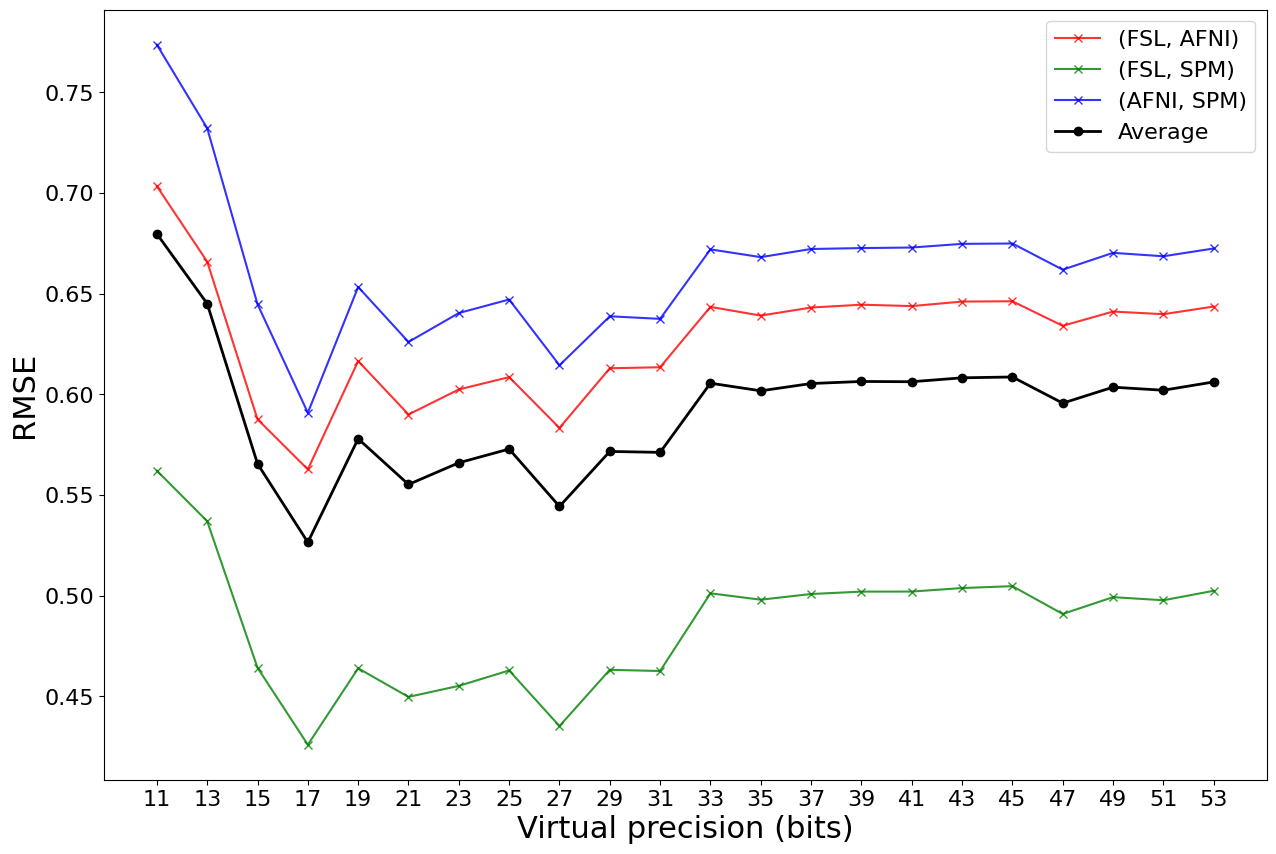
\includegraphics[width=\columnwidth]{figures/rmse-precisions.png}
        %\caption{Standard deviation of thresholded t-statistics map on template surface}
      \caption{Comparison of RMSE values computed between BT and WT resulted from FSL tool for different virtual precisions \tristan{Make a full figure, similar to Fig 5, 3, and 1.}.}
    \label{fig:across-precisions}
    \end{minipage}}
  \end{figure}

  
  %%%%%%%%%% plot different precisions%%%%%%%%
  \begin{figure}[ht]
    \fbox{\begin{minipage}{\dimexpr \columnwidth-2\fboxsep-2\fboxrule}
        \centering
        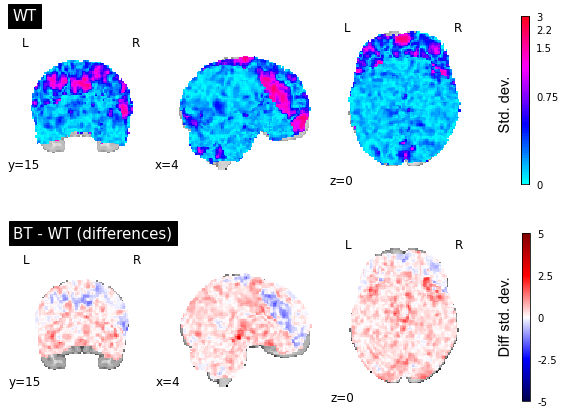
\includegraphics[width=\columnwidth]{figures/bt-wt.png}
        %\caption{Standard deviation of thresholded t-statistics map on template surface}
      \caption{Comparison of standard deviations in BT averaged across pairs of tools and WT resulted from FSL tool
      at the virtual precision of t=27 bits.}
    \label{fig:gnp-mni}
    \end{minipage}}
  \end{figure}



\section{Discussion}

\begin{itemize}

  \item[$\bullet$ ] In this study, we represented the magnitude of differences in BT and WT results.
  We obtained more instability in BT compared to WT. Also we showed how between tool variations
  are correlated with numerical variability.
  While we only perturbed basic mathematical functions, perturbing linear algebra, in particular, could increase WT variability.

  \item[$\bullet$ ] Generally, we obtained more uncertainty on thresholded results, probably due to different thresholding
  methods used in different tools. This can raise further investigations on the thresholding techniques toward stability.
  Also, we obtained significant instabilities in specific subjects so that healed by averaging in group-level analyses.

  \item[$\bullet$ ] We showed that reducing the number of virtual precision bits leads to more instabnilities in which can exceeds variability compared to BT.
  We also showed the numerical perturbations can perfectly simulate BT variability in some regions. 
   
  \item[$\bullet$] Numerical instability in individual analyses is attenuated in group analyses. This is an issue for the development of fMRI biomarkers.
  \item[$\bullet$] Comparision between FSL, SPM and AFNI. Discussion on the instrumentation of math functions only.
\end{itemize}



% There are many statistical comparisons, but the neuro-scientific interpretation of results is not on my side.

\section{Conclusion}

\begin{itemize}

    \item[$\bullet$ ] Further studies can be evaluating the numerical stabilities within tool by focusing on the particular parts of
    the pipeline that has been identified as the main sources of variations in~\cite{bowring2021isolating}.
    Also, we can invetigate the precision in WT variability that simulates mostly BT variability in the furure study.

\end{itemize}


\section{Acknowledgments}


%%
%% The next two lines define the bibliography style to be used, and
%% the bibliography file.
\bibliographystyle{plain}
\bibliography{biblio}


\end{document}
\endinput
%%
%% End of file `sample-authordraft.tex'.
